
\chapter{今後の課題:提案手法の遅延}
\label{sec:appendix2}
本研究における未解決の課題である,提案手法におけるウェイクアップ時の遅延に関して説明する.

提案手法にはウェイクアップ論理の遅延が増加するという問題がある.これは,ウェイクアップ論理のクリティカル・パスに SVSD での SVS の生成と,タグの高位ビットと SVS との論理積が加わるためである.一般に,ウェイクアップ論理はプロセッサ全体のクリティカル・パスであるため,ウェイクアップ論理の遅延増加は,クロック・サイクル時間の増加につながり,結果として性能が低下する.したがって,提案手法によるウェイクアップ論理の遅延の増加は許容できる範囲に抑える必要がある.

SVSD での遅延の影響を測定するために,HSPICE による回路シミュレーションにより測定を行った.16nm LSI プロセスを仮定し,トランジスタ・モデルとして,アリゾナ州立大学のPredictiveTechnology Model(PTM)~\cite{model2012}を使用した.International Technology Roadmap for Sem-conductors(ITRS)~\cite{itrs2012}により公開されているデータより,単位長さあたりの配線抵抗は 46.96MΩ/m,配線容量は 0.165nF/m とした.なお,この HSPICE による回路シュミレーションは,松田~\cite{matsuda-thesis}の作成したネットリスト生成プログラム及び遅延測定用スクリプトを修正して使用することにより行った. 

測定を行った SVSD 回路の回路図を\fig{SVSD_nand_nor}に示す.当図は,セグメント数が 8 で,タグのビット数が 8 ビットの場合を示している.基本的な回路構成は\refsec{segment_IQ}で説明したものと同様であるが,CMOS トランジスタで構成するため,NAND 及び NOR を使用する回路構成に変更している.本回路に関して詳しく説明する.

\ctext{1}SVSD は,ディスティネーション・タグの下位 3 ビットの正転及び反転信号を用いて,セグメント数分の SVS の反転信号 $\lnot SVS$ を生成する.\ctext{2} $\lnot SVS$ は,ディスティネーション・タグの反転(正転)信号と否定論理和をとり,SVS によって有効化されたディスティネーション・タグ(v-dtag:validated dtag)の正転(反転)信号を生成する.これは,以下の論理式に基づいている.
\[
  v\_dtag = \lnot (\lnot dtag \lor \lnot SVS) \; (= dtag \land SVS) 
\]
\[
  \lnot v\_dtag = \lnot (dtag \lor \lnot SVS) \; (= \lnot dtag \land SVS) 
\]

  松田のネットリスト生成プログラムを修正して,SVS を含む提案手法のウェイクアップ回路の遅延測定を行った.測定結果を表の各期間は次の意味を持つ.
  \begin{itemize}
    \item from tagRAM:タグRAM から SVS  の入力まで
    \item SVS:SVS 信号の生成(\fig{SVSD_nand_nor}における赤い矢印)
    \item broadcast:SVS により有効化したタグのブロードキャスト(CAM の入力まで)(\fig{SVSD_nand_nor}における青い矢印) 
  \end{itemize}

  \begin{table}[htb]
    \caption{ウェイクアップ論理の遅延時間(ps)}
    \footnotesize
    \center
      \begin{tabular}{l|l} \hline \hline
       from tagRAM & 24.849 \\
       SVS & 36.192 \\
       broadcast & 105.72 \\ \hline
    \end{tabular}
    \label{tab:delay}
  \end{table}

  評価の結果,その結果,SVS 信号の遅延(\fig{SVSD_nand_nor}における赤い矢印)が想定していたよりも大幅に大きかった.提案手法を用いない場合の通常の IQ におけるタグのブロードキャストの遅延時間を評価したところ,120ps 程度であったため,36p という遅延の増加は無視できないほど大きい.この原因は特定できていないが,おそらく SVSD の NAND ゲートへの入力信号の立ち上がりが遅いためではないかと予測している.

  この問題への対処方法としては,タグ RAM に SVSD を配置し, SVS に変換してからブロードキャストする方法や,ディスパッチ時にあらかじめ SVS に変換してタグ RAM に記録しておき,ブロードキャスト時に タグとともにブロードキャストする方法などが考えられる.これらの方法について検討し,ウェイクアップ論理の遅延増加を許容できる範囲に抑えることが今後の課題である.
  
\begin{figure}[htb]
  \centering
  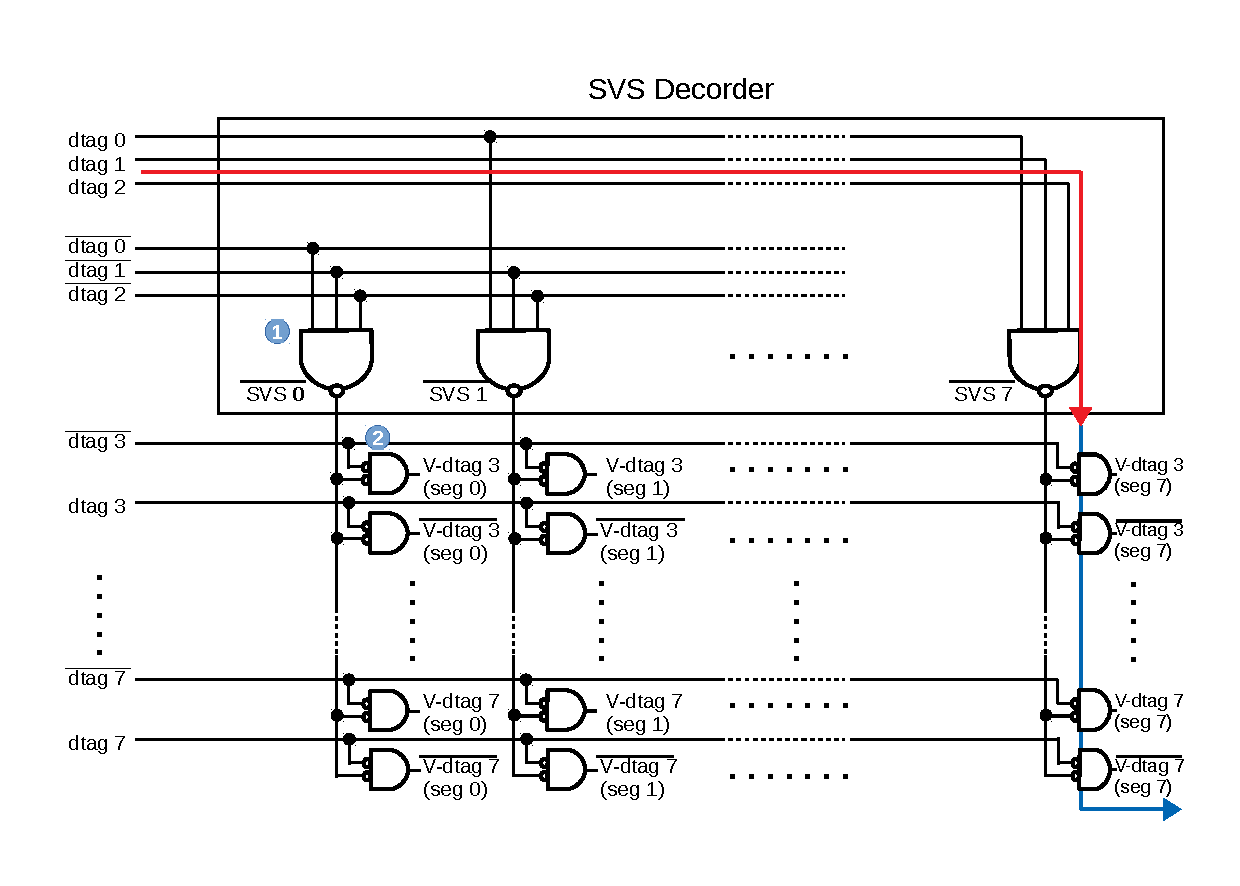
\includegraphics[keepaspectratio, scale=.8]{SVSD_nand_nor}
  \caption{SVSD(遅延評価用)}
  \label{fig:SVSD_nand_nor}
\end{figure}
